\setcounter{chapter}{13}
\chapter{Survival Models}

{\small \textit{Chapter Preview}. This chapter introduces regression
where the dependent variable is the time until an event, such as the
time until death, onset of a disease or the default on a loan. Event
times are often limited by sampling procedures and so ideas of
censoring and truncation of data are summarized in this chapter.
Event times are non-negative and their distributions are described
in terms of survival and hazard functions. Two types of hazard-based
regression are considered, a fully parametric accelerated failure
time model and a semi-parametric proportional hazards models.}

\section{Introduction}

In survival models, the dependent variable is the time until an
event of interest. The classic example of an event is time until
death (the complement of death being survival). Survival models are
now widely applied in many scientific disciplines; other examples of
events of interest include the onset of Alzheimer's disease
(biomedical), time until bankruptcy (economics) and time until
divorce (sociology).

\linejed\index{examples!time until bankruptcy}\index{actuarial \&
financial terms and concepts!bankruptcy}

\textbf{Example: Time until Bankruptcy.}\ecaptionjed{Time until
Bankruptcy} Shumway (2001) examined the time to bankruptcy for 3,182
firms listed on Compustat Industrial File and the CRSP Daily Stock
Return File for the New York Stock Exchange over the period
1962-1992. Several explanatory financial variables were examined,
including working capital to total assets, retained earnings to
total assets, earnings before interest and taxes to total assets,
market equity to total liabilities, sales to total assets, net
income to total assets, total liabilities to total assets and
current assets to current liabilities. The data set included 300
bankruptcies from 39,745 firm years.

See also Kim et al. (1995) for a similar study on insurance
insolvencies.

\linejed\index{censoring}\index{truncated}

\marginparjed{A distinguishing feature of survival modeling is that
dependent variables are often limited by censoring and truncation.}

A distinguishing feature of survival modeling is that it is common
for the dependent variable to be observed only in a limited sense.
Some events of interest, such as bankruptcy or divorce, never occur
for specific subjects (and so can be thought of as taking an
infinite time). For other subjects, even when the event time is
finite, it may occur after the study period so that the data are
(right) \emph{censored}. That is, complete information about event
times may not be available due to the design of the study. Moreover,
firms may merge with or be acquired by other firms and individuals
may move from a geographical area, leaving the study. Thus, the data
may be limited by events that are extraneous to the research
question under consideration, represented as \emph{random}
censoring. Censoring is a regular feature of survival data; large
values of a dependent variable require more time to develop so that
they can be more difficult to observe than small values, other
things being equal. Other types of limitations may also occur;
subjects whose observation depends on the experience of the event of
interest are said to be \emph{truncated}. To illustrate, in an
investigation of old-age mortality, only those who survive to age 85
are recruited to be a part of the study. Section
\ref{S14:CensoringTruncation} describes censoring and truncation in
more detail.


Another distinguishing feature of survival modeling is that the
dependent variable is positive-valued. Thus, normal curve
approximations used in linear regression are less helpful in
survival analysis; this chapter introduces alternative regression
models. Further, it is customary to interpret models of survival
using the \emph{hazard function}, defined as
\begin{eqnarray*}
\mathrm{h}(t)&= &\frac{probability~density~function}
{survival~function} =\frac{\mathrm{f}(t)}{\mathrm{S}(t)},
\end{eqnarray*}
the ``instantaneous'' probability of an event, conditional on
survivorship up to time $t$. The hazard function goes by many other
names: it is known as the \emph{force of mortality} in actuarial
science, the \emph{failure rate} in engineering and the
\emph{intensity function} in stochastic processes.

\marginparjed{Duration dependence describes the relation between the
instantaneous event probability and the time spent in a given
state.}

In economics, hazard functions are used to describe \textit{duration
dependence}, the relation between the instantaneous event
probability (the density) and the time spent in a given state.
\textit{Negative} duration dependence is associated with decreasing
hazard rates. For example, the longer the time until a claimant
requests a payment from an insured injury, the lower is the
probability of making a request. \textit{Positive} duration
dependence is associated with increasing hazard rates. For example,
old-age human mortality generally displays an increasing hazard
rate. The older someone is, the higher the near-term probability of
death.

A related quantity of interest is the \emph{cumulative hazard
function}, $H(t)= \int_0^t h(s)ds$. This quantity can also be
expressed as the negative log survival function, and conversely,
$\Pr(y>t)=\mathrm{S}(t) = \exp (-H(t))$.

The two most widely used regression models in survival analysis are
based on hazard functions. Section \ref{S14:AFT} introduces the
\emph{accelerated failure time model}, where one assumes a linear
model for the logarithmic time to failure but with an error
distribution that need not be approximately normal. Section
\ref{S14:Cox} introduces the the \emph{proportional hazards model}
due to Cox (1972), where one assumes that the hazard function can be
written as the product of a ``baseline'' hazard and a function of a
linear combination of explanatory variables.

With survival data we observe a cross-section of subjects where time
is the dependent variable of interest. As with Chapter 10 on
longitudinal and panel data, there are also applications in which we
are interested in repeated observations for each subject. For
example, if you are injured in an accident that is covered by
insurance, the payments that arise from this claim can occur
repeatedly over time, depending on the time to recovery. Section
\ref{S14:RecurrentEvents} introduces the notion of repeated event
times, called \emph{recurrent events}.



\section{Censoring and Truncation}\label{S14:CensoringTruncation}

\subsection{Definitions and Examples}

Two types of limitations encountered in survival data are
\emph{censoring} and \emph{truncation}. Censoring and truncation are
also common features in other actuarial applications, including the
Chapter 16 two-part and Chapter 17 fat-tailed models. Thus, this
section describes these concepts in detail.

For censoring, the most common form is \emph{right-censoring}, in
which we observe the smaller of the ``true'' dependent variable and
a censoring time variable. For example, suppose that we wish to
study the time until a new employee leaves the firm and that we have
five years of data to conduct our analysis. Then, we observe the
smaller of five years and the amount of time that the employee was
with the firm. We also observe whether or not the employee has
departed within five years.

Using notation, let $y$ denote the time to the event, such as the
amount of time the employee worked with a firm. Let $C_U$ denote the
censoring time, such as $C_U=5$. Then, we observe the variable
$y_U^{\ast}= \min(y, C_U)$. We also observe whether or not censoring
has occurred. Let  $\delta_U= \mathrm{I}(y \geq C_U)$ be a binary
variable that is 1 if censoring occurs, $y \geq C_U$, and 0
otherwise. For example, in Figure \ref{F14:Censoring}, values of $y$
that are greater than the ``upper'' censoring limit $C_U$ are not
observed -- thus, this is often called \emph{right-censoring}.


\begin{figure}[htp]
  \begin{center}
    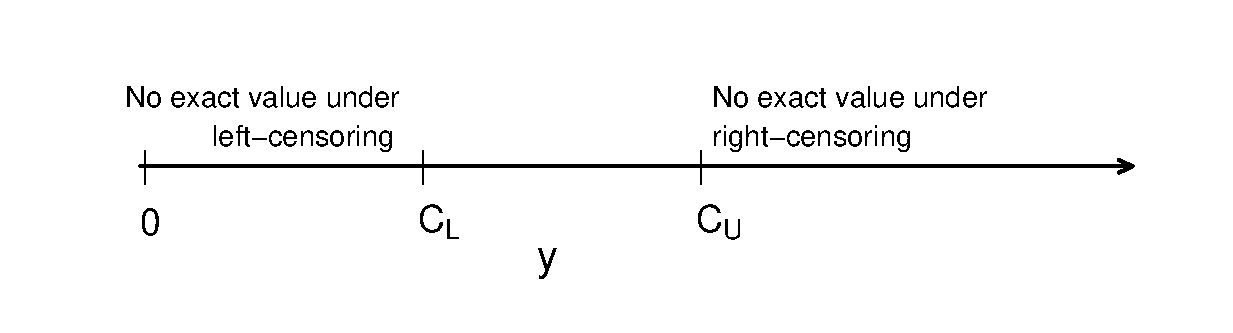
\includegraphics[width=.8\textwidth]{Chapter14Survival/F14CensoringA.eps}
    \caption{\label{F14:Censoring}\small Figure Illustrating Left- and Right-Censoring.}
  \end{center}
\end{figure}


Other common forms of censoring are \textit{left-censoring} and
\textit{interval censoring}. With left-censoring, we observe
$y_L^{\ast}= \max(y, C_L)$ and $\delta_L= \mathrm{I}(y \leq C_L)$
where $C_L$ is the censoring time. For example, if you are
conducting a study and interviewing a person about an event in the
past, the subject may recall that the event occurred before $C_L$
but not the exact
date.\index{censoring!left-}\index{censoring!right-}\index{censoring!interval}

\marginparjed{Common forms of censoring include left-, right- and interval censoring.}

With interval censoring, there is an interval of time, such as
$(C_L, C_U)$, in which $y$ is known to occur but the exact value is
not observed. For example, you may be looking at two successive
years of annual employee records. People employed in the first year
but not the second have left sometime during the year. With an exact
departure date, you could compute the amount of time that they were
with the firm. Without the departure date, then you only know that
they departed sometime during a year-long interval.


\marginparjed{
\newline
\newline
\newline
\newline
Censoring times may be fixed or random. Fixed and independent random
censoring are said to be
non-informative.}\index{censoring!fixed}\index{censoring!random}

Censoring times such as $C_L$ and $C_U$ may or may not be
stochastic. If the censoring times represent variables known to the
analyst, such as the observation period, they are said to be
\emph{fixed censoring} times. Here, the adjective ``fixed'' means
that the times are known in advance. Censoring times may vary by
individual but still be fixed. However, censoring may also be the
result of an unforeseen phenomena, such as firm merger or a subject
moving from a geographical area. In this case, the censoring $C$ is
represented by a random variable and said to be \emph{random
censoring}. If the censoring is fixed or if the random censoring
time is independent of the event of interest, then the censoring is
said to be \emph{non-informative}. If the censoring times are
independent of the event of interest, then we can essentially treat
the censoring as fixed. When censoring and the time to event are
dependent (known as \emph{informative censoring}), then special
models are required. For example, if the event of interest is time
until bankruptcy of a firm and the censoring mechanism involves
filing adequate financial statements, then there is a potential
relationship. Financially weak firms are more likely to become
bankrupt and less likely to go through the accounting effort to file
adequate statements.

Censored observations are available for study, although in a limited
form. In contrast, \emph{truncated} responses are a type of missing
data. To illustrate, with \emph{left-truncated }data, if $y$ is less
than a threshold (say, $C_L$), then it is not observed. For
\emph{right-truncated} data, if $y$ exceeds a threshold (say,
$C_U$), then it is not observed. To compare truncated and censored
observations, consider the following
example.\index{truncated!right-}\index{truncated!left-}

\linejed

\begin{figure}[htp]
  \begin{center}
    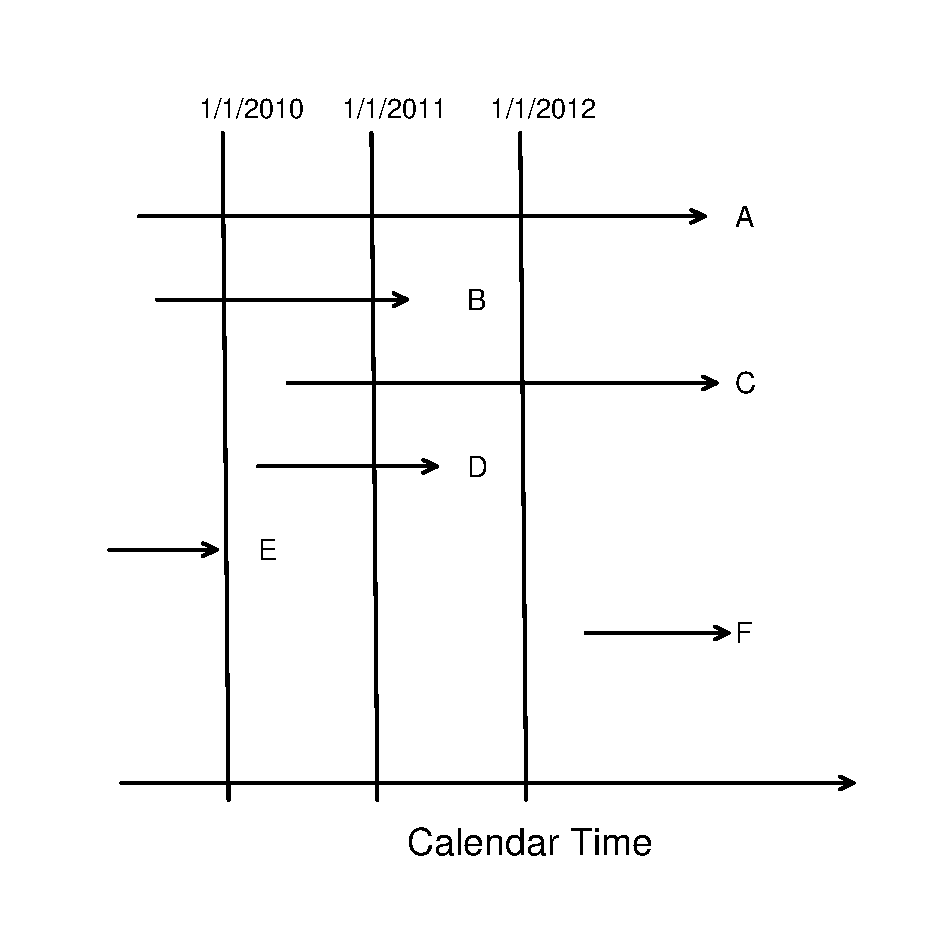
\includegraphics[width=.6\textwidth]{Chapter14Survival/F14Mortality.eps}
    \caption{\label{F14:Mortality}\small Timeline for Several Subjects in a Mortality Study.}
  \end{center}
\end{figure}


\textbf{Example: Mortality Study.} Suppose that you are conducting a
two-year study of mortality of high-risk subjects, beginning January
1, 2010 and finishing January 1, 2012. Figure \ref{F14:Mortality}
graphically portrays the six types of subjects recruited. For each
subject, the beginning of the arrow represents that the the subject
was recruited and the arrow end represents the event time. Thus, the
arrow represents exposure time.


\begin{itemize}
\item Type A - right-censored. This subject is alive at the beginning and the end of
the study. Because the time of death is not known by the end of the
study, it is right-censored. Most subjects are Type A.
\item Type B. Complete information is available for a type B subject. The subject is
alive at the beginning of the study and the death occurs within the
observation period.
\item Type C - right-censored and left-truncated. A type C subject is right-censored,
in that death occurs after the observation period. However, the
subject entered after the start of the study and is said to have a
\emph{delayed entry time}. Because the subject would not have been
observed had death occurred before entry, it is left-truncated.
\item Type D - left-truncated. A type D subject also has delayed entry.
Because death occurs within the observation period, this subject is
not right censored.
\item Type E - left-truncated. A type E subject is not included in the study because
death occurs prior to the observation period.
\item Type F - right-truncated. Similarly, a type F subject is not included because the entry time
occurs after the observation period.
\end{itemize}

\linejed

\subsection{Likelihood Inference}\index{likelihood
inference!censoring}

Many inference techniques for survival modeling involve likelihood
estimation, so it is helpful to understand the implications of
censoring and truncation when specifying likelihood functions. For
simplicity, we assume fixed censoring times and a continuous time to
event $y$.

To begin, consider the case of right-censored data where we observe
$y_U^{\ast}= \min(y, C_U)$ and $\delta_U= \mathrm{I}(y \geq C_U)$.
If censoring occurs so that $\delta_U=1$, then $y \geq C_U$ and the
likelihood is $ \Pr(y \geq C_U) = \mathrm{S}(C_U)$. If censoring
does not occur so that $\delta_U=0$, then $y < C_U$ and the
likelihood is $\mathrm{f}(y)$. Summarizing, we have
\begin{eqnarray*}
Likelihood  &=& \left\{
\begin{array}{cl}
\mathrm{f}(y) & \textrm{if~}\delta=0 \\
\mathrm{S}(C_U)  &  \textrm{if~}\delta=1
\end{array}
\right. \\&=& \left( \mathrm{f}(y)\right)^{1-\delta} \left(
\mathrm{S}(C_U)\right)^{\delta} .
\end{eqnarray*}
The right-hand expression allows us to present the likelihood more
compactly. Now, for an independent sample of size $n$, $\{ (y_{U1},
\delta_1), \ldots,(y_{Un}, \delta_n) \} $, the likelihood is
\begin{equation*}
\prod_{i=1}^n \left( \mathrm{f}(y_i)\right)^{1-\delta_i} \left(
\mathrm{S}(C_{Ui})\right)^{\delta_i} = \prod_{\delta_i=0}
\mathrm{f}(y_i) \prod_{\delta_i=1} \mathrm{S}(C_{Ui}),
\end{equation*}
with potential censoring times $\{ C_{U1},  \ldots,C_{Un} \} $.
Here, the notation ``$\prod_{\delta_i=0}$'' means take the product
over uncensored observations, and similarly for
``$\prod_{\delta_i=1}$.''

Truncated data are handled in likelihood inference via conditional probabilities.
Specifically, we adjust the likelihood contribution by dividing by the probability
that the variable was observed. Summarizing, we
have the following contributions to the likelihood for six types of
outcomes.
\begin{center}
\scalefont{0.9}
\begin{tabular}{lc}
\hline Outcome            & Likelihood~Contribution \\\hline
exact~value        & f($y$) \\
right-censoring    & S($C_U$) \\
left-censoring     & 1-S($C_L$) \\
right-truncation   & f($y$)/(1-S($C_U$)) \\
left-truncation    & f($y$)/S($C_L$) \\
interval-censoring & S($C_L$)-S($C_U$) \\
\hline
\end{tabular}
\scalefont{1.1111}
\end{center}

For known event times and censored data, the likelihood is
\begin{equation*}
\prod_{E} \mathrm{f}(y_i) \prod_{R} \mathrm{S}(C_{Ui}) \prod_{L}
(1-\mathrm{S}(C_{Li})) \prod_{I}
(\mathrm{S}(C_{Li})-\mathrm{S}(C_{Ui})),
\end{equation*}
where ``$\prod_{E}$'' is the product over observations with
\textit{E}xact values, and similarly for \textit{R}ight-,
\textit{L}eft- and \textit{I}nterval-censoring.

For right-censored and left-truncated data, the likelihood is
\begin{equation*}
\prod_{E} \frac{\mathrm{f}(y_i)}{\mathrm{S}(C_{Li})} \prod_{R}
\frac{\mathrm{S}(C_{Ui})}{\mathrm{S}(C_{Li})} ,
\end{equation*}
and similarly for other combinations. To get further insights,
consider the following.

\linejed\index{distributions!exponential}

\textbf{Special Case: Exponential Distribution.} Consider data that
are right-censored and left-truncated, with dependent variables
$y_i$ that are exponentially distributed with mean $\mu$. With these
specifications, recall that $\mathrm{f}(y) = \mu^{-1} \exp(-y/\mu)$
and $\mathrm{S}(y) = \exp(-y/\mu)$.

For this special case, the logarithmic likelihood is
\begin{eqnarray*}
 \ln Likelihood  &=& \sum_{E} \left( \ln \mathrm{f}(y_i) - \ln
\mathrm{S}(C_{Li}) \right)
 +\sum_{R}\left( \ln \mathrm{S}(C_{Ui})- \ln \mathrm{S}(C_{Li})
 \right) \\
 &=&  \sum_{E} (-\ln \mu -(y_i-C_{Li})/\mu )
-\sum_{R} (C_{Ui}-C_{Li})/\mu .
\end{eqnarray*}
To simplify the notation, define $\delta_i = \mathrm{I}(y_i \geq
C_{Ui})$ to be a binary variable that indicates right-censoring. Let
$y_i^{\ast \ast} = \min(y_i, C_{Ui}) - C_{Li}$ be the amount that
the observed variable exceeds the lower truncation limit. With this,
the logarithmic likelihood is
\begin{equation}\label{E14:ExponentialLike}
 \ln Likelihood =  - \sum_{i=1}^n ((1-\delta_i) \ln \mu + \frac{y_i^{\ast
 \ast}}{\mu} ).
\end{equation}
Taking derivatives with respect to the parameter $\mu$ and setting
it equal to zero yields the maximum likelihood estimator
\begin{eqnarray*}
\widehat{\mu}
 &=& \frac{1}{n_u} \sum_{i=1}^n  y_i^{\ast
 \ast},
\end{eqnarray*}
where $n_u = \sum_i (1-\delta_i)$ is the number of uncensored
observations.

\linejed


\subsection{Product-Limit Estimator}\index{product-limit estimator}

It can be useful to calibrate likelihood methods with nonparametric
methods that do not rely on a parametric form of the distribution.
The \emph{product-limit estimator }due to Kaplan and Meier (1958) is
a well-known estimator of the distribution in the presence of
censoring.

To introduce this estimator, we consider the case of
right-censored data. Let $t_1 < \cdots < t_c$ be distinct time
points at which an event of interest occurs and let $d_j$ be the
number of events at time point $t_j$. Further, define $R_j$ to be
the corresponding ``risk set'' - this is the number of observations
that are active at an instant just prior to $t_j$. Using notation,
the risk set is $R_j = \sum_{i=1}^n I\left( y_i \geq
 t_j \right)$. With this notation, the product-limit estimator of
the survival function is
\begin{equation}\label{E14:ProductLimit}
\widehat{S}(t) = \left\{
\begin{array}{ll}
 1 & t<t_1 \\
  \prod_{t_j \leq t} \left(1 - \frac{d_j}{R_j}
\right)
   & t \geq t_1
\end{array}
\right. .
\end{equation}

To interpret the product-limit estimator, we look to evaluating it
at event times. At the first event time $t_1$, the estimator is
$\widehat{S}(t_1)= 1- d_1/R_1=(R_1 - d_1)/R_1$, the proportion of
non-events from the risk set $R_1$. At the second event time $t_2$,
the survival probability conditional on survivorship to time $t_1$
is $\widehat{S}(t_2)/ \widehat{S}(t_1)= 1 - d_2/R_2=(R_2 -
d_2)/R_2$, the proportion of non-events from the risk set $R_2$.
Similarly, at  the $j$th event time,
\begin{equation*}\frac{\widehat{S}(t_j)}{\widehat{S}(t_{j-1})}= 1 - \frac{d_j}{R_j}=\frac{R_j -
d_j}{R_j} .
\end{equation*}
Starting from these conditional probabilities, one can build the
survival estimate as

\begin{equation*}
\widehat{S}(t_j) = \frac{\widehat{S}(t_j)}{\widehat{S}(t_{j-1})}
\times \cdots \times \frac{\widehat{S}(t_2)}{\widehat{S}(t_{1})}
\times \widehat{S}(t_{1}),
\end{equation*}
resulting in equation (\ref{E14:ProductLimit}). In this sense, the
estimator is a ``product,'' up to the time ``limit.'' For times
between event times, the survival estimate is taken to be a
constant.

To see how to use the product-limit estimator, we consider a small
data set of $n=23$ observations, where 18 are event times and 5 have
been right-censored. This example is from Miller (1997), where the
events correspond to survival for patients with acute myelogenous
leukemia. After patients received chemotherapy to achieve complete
remission, they were randomly allocated to one of two groups, those
who received maintenance chemotherapy and those who did not (the
control group). The event was time in weeks to relapse from the
complete remission state. For those in the maintenance group, the
times are: 9, 13, 13+, 18, 23, 28+, 31, 34, 45+, 48, 161+. For those
in the control group, the times are: 5, 5, 8, 8, 12, 16+, 23, 27,
30, 33, 43 45. Here, the plus sign (+) indicates right-censoring of
an observation.

Figures \ref{F14:ProductLimitA} and \ref{F14:ProductLimitB} show the
product-limit survival function estimates for these data. Notice the
step nature of the function, where drops (from the left, or jumps
from the right) correspond to event times. When no censoring is
involved, the product-limit estimator reduces to the usual empirical
estimator of the survival function.

In the figures, censored observations are depicted with a plus (+)
plotting symbol. When the last observation has been censored as in
Figure \ref{F14:ProductLimitA}, there are different methods for
defining the survival curve for times exceeding this observation.
Analysts making estimates at these times will need to be aware of
the option that their statistical package uses. The options are
described in standard books on survival analysis, such as Klein and
Moschberger (1997).


\begin{figure}[htp]
    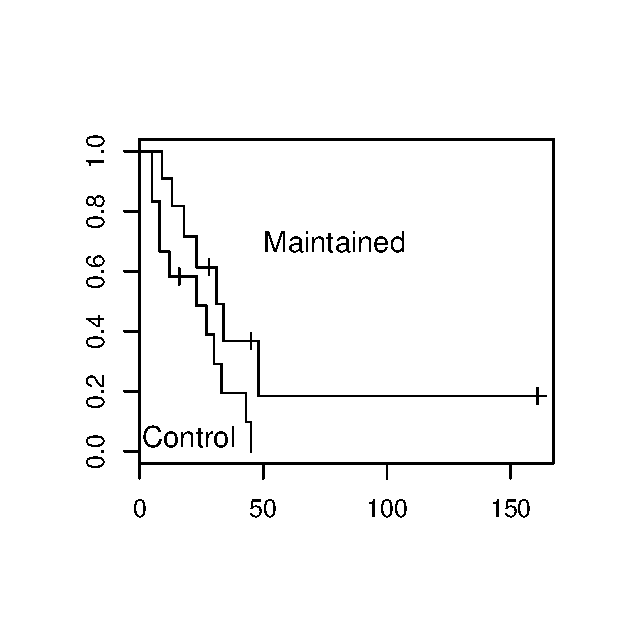
\includegraphics[width=0.45\textwidth]
        {Chapter14Survival/F14ProductLimitA.eps} \hfill  $~~~$
               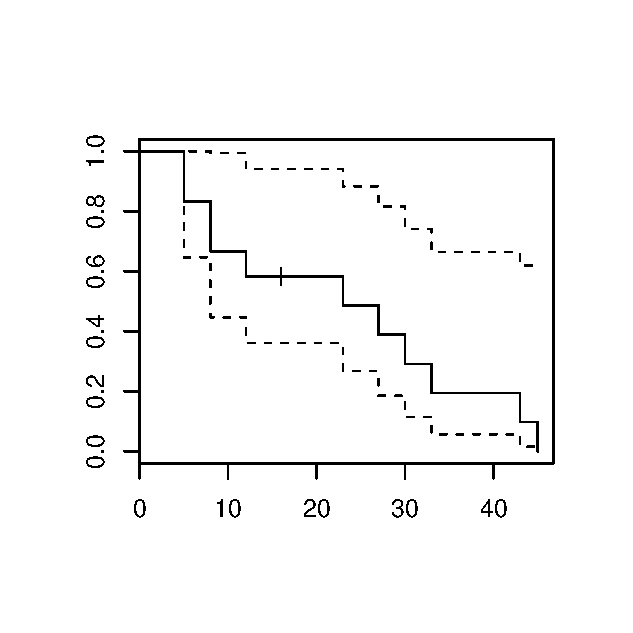
\includegraphics[width=0.45\textwidth]
        {Chapter14Survival/F14ProductLimitB.eps}

      \parbox[t]{2.5in}{\caption{\label{F14:ProductLimitA} \small Product-Limit
      Estimate of the Survival Functions for Two Groups.
      This graph shows that those with maintained chemotherapy treatment
      have higher estimated survival probabilities than those in the control group.}} \hfill
        \parbox[t]{2.5in}{\caption{\label{F14:ProductLimitB} \small Product-Limit
        Estimate of the Survival Function for the Control Group.
    The upper and lower bounds are from Greenwood's formula for the estimate of the variance.}}
\end{figure}

Figure \ref{F14:ProductLimitB} also shows an estimate of the
standard error. These are calculated using Greenwood's (1926)
formula for an estimate of the variance, given by
\begin{equation*}
\widehat{\mathrm{Var}(\widehat{S}(t))} = (\widehat{S}(t))^2
  \sum_{t_j \leq t}  \frac{d_j}{R_j(R_j-d_j)} .
\end{equation*}


\section{Accelerated Failure Time
Model}\label{S14:AFT}\index{regression model!accelerated failure
time, $AFT$}

An accelerated failure time ($AFT$) model can be expressed using a
linear regression equation $ \ln y_i = \mathbf{x}_i^{\prime}
\boldsymbol \beta + \varepsilon_i $, where $y_i$ is the event time.
Unlike the usual linear regression model, the AFT model makes a
parametric assumption about the disturbance term, such as a normal,
extreme-value or logistic distribution. As we have seen, the normal
distribution is the basis for usual linear regression model. Thus,
many analysts begin by taking logarithms of event data and using the
usual linear regression routines to explore their data.

\subsubsection*{Location-Scale
Distributions}\index{distributions!location-scale}

To understand the name ``accelerated failure,'' also known as
accelerated hazards, it is helpful to review the statistical idea of
location-scale families. A parametric \emph{location-scale
distribution} is one where the density function is of the form
\begin{equation*}
\mathrm{f}(t) =\frac{1}{\sigma }\mathrm{f}_0 \left( \frac{t-\mu
}{\sigma }\right) ,
\end{equation*}
where $\mu $ is the location parameter and $\sigma >0$ is the scale
parameter. The case $\mu =0$\ and $\sigma =1$\ corresponds to the
\emph{standard form} of the distribution. Within a location-scale
distribution, additive shifts, such as going from degrees Kelvin to
degrees Centigrade, $^{\circ }K=$ $^{\circ }C+273.15$, and scalar
multiples, such as going from dollars to thousands of dollars,
remain in the same distribution family. As we will see in Chapter
17, a location parameter is a natural place to introduce regression
covariates.\index{distributions!log location-scale}

A random variable $y$ is said to have a \emph{log location-scale
distribution} if $\ln y$ has a location-scale distribution. Suppose
that a random variable $y_0$ has a standard form location-scale
distribution with survival function $\mathrm{S}_0\left( z\right) $.
Then, the survival function of $y$ defined by $\ln y = \mu + \sigma
y_0$ can be expressed as
\begin{equation*}
\mathrm{S}\left( t\right) =\Pr \left( y>t\right) =\Pr \left(
y_0>\frac{\ln t-\mu }{\sigma }\right) =\mathrm{S}_0\left( \frac{\ln
t-\mu }{\sigma } \right) =\mathrm{S}_0^{\ast }\left( \left(
\frac{t}{e^{\mu }}\right) ^{1/\sigma }\right) ,
\end{equation*}
where $\mathrm{S}_0^{\ast }(t) =\mathrm{S}_0( \ln t) $ is the
survival function of the standard form of $\ln y$. In the context of
survival modeling where $t$ represents time, the effect of rescaling
by dividing by $e^{\mu }$ can be thought of as ``accelerating time''
(when $e^{\mu }<1$). This is the motivation for the name
``accelerated failure time models.'' Table
\ref{T14:LocationScaleDist} provides some special cases of widely
used location-scale distributions and their log location-scale
counterparts.

\index{distributions!Weibull}\index{distributions!extreme value}
\index{distributions!log-normal}\index{distributions!logistic}

\begin{table}[h]
\scalefont{0.9} \caption{\label{T14:LocationScaleDist}
Location-Scale Distributions}
\begin{equation*}
\begin{tabular}{ccc}
\hline
Standard Form & Location-Scale & Log Location-Scale \\
Survival Distribution & Distribution & Distribution \\ \hline
$\mathrm{S}_0(t) =\exp \left( -e^t \right) $ & extreme value
distribution & Weibull \\
$\mathrm{S}_0(t) =1 - \Phi(t) $ & normal &
log-normal \\
$\mathrm{S}_0(t) = (1 + e^t)^{-1}$ & logistic & log-logistic \\
\hline
\end{tabular}
\end{equation*}
\scalefont{1.1111}
\end{table}

\subsubsection*{Inference for AFT Models}\index{likelihood
inference!accelerated failure time model}

To get an idea of the complexities in estimating an $AFT$ model, we
return to the exponential distribution. This is a special case of
Weibull regression with the scale parameter $\sigma =1$.


\linejed

\textbf{Special Case: Exponential Distribution - Continued.} To
introduce regression covariates, we let $\mu_i = \exp
(\mathbf{x}_i^{\prime} \boldsymbol \beta)$. Using the same reasoning
as with equation (\ref{E14:ExponentialLike}), the logarithmic
likelihood is
\begin{eqnarray*}
 \ln Likelihood
 &=&  - \sum_{i=1}^n ((1-\delta_i) \ln \mu_i +\frac{y_i^{\ast
 \ast}}{\mu_i} )\\
 &=&  - \sum_{i=1}^n ((1-\delta_i) \mathbf{x}_i^{\prime} \boldsymbol \beta+ y_i^{\ast
 \ast}\exp
(-\mathbf{x}_i^{\prime} \boldsymbol \beta)) ,
\end{eqnarray*}
where $\delta_i = I(y_i \geq C_{Ui})$ and $y_i^{\ast \ast} =
\min(y_i, C_{Ui}) - C_{Li}$. Taking derivatives with respect to
$\boldsymbol \beta$ yields the score function
\begin{eqnarray*}
\frac{\partial \ln Likelihood}{\partial \boldsymbol \beta}
 &=&  - \sum_{i=1}^n ((1-\delta_i) \mathbf{x}_i - \mathbf{x}_i y_i^{\ast
 \ast}\exp
(-\mathbf{x}_i^{\prime} \boldsymbol \beta)) \\
 &=&    \sum_{i=1}^n  \mathbf{x}_i
\frac{y_i^{\ast
 \ast}-\mu_i (1-\delta_i)}
{\mu_i } .
\end{eqnarray*}
This has the form of a generalized estimating equation, introduced
in Chapter 13. Although closed-form solutions rarely exist, it can
readily be solved by modern statistical packages.

\linejed

As this special case illustrates, estimation of $AFT$ regression
models can be readily addressed through maximum likelihood.
Moreover, properties of maximum likelihood estimates are
well-understood and so we readily have general inference tools, such
as estimation and hypothesis testing, available. Standard
statistical packages provide output that supports this inference.


\section{Proportional Hazards Model}\label{S14:Cox}\index{regression model!proportional hazards, $PH$}

The assumption of proportional hazards is defined in Section
\ref{S14:PHAssumption} and inference techniques are discussed in
Section \ref{S14:PHInference}.

\subsection{Proportional Hazards}\label{S14:PHAssumption}


In the \emph{proportional hazards} ($PH$) model due to Cox (1972),
one assumes that the hazard function can be written as the product
of some ``baseline'' hazard and a function of a linear combination
of explanatory variables. To illustrate, we use
\begin{equation}\label{E14:PHHazardFunction}
h_i(t) = h_0(t) \exp( \mathbf{x}_i^{\prime} \boldsymbol \beta ).
\end{equation}
where $h_0(t)$ is the baseline hazard. This is known as a
``proportional'' hazards model because if one takes the ratio of
hazard functions for two sets of covariates, say $\mathbf{x}_1$ and
$\mathbf{x}_2$, one gets
\begin{equation*}
\frac{h_1(t|\mathbf{x}_1)}{h_2(t|\mathbf{x}_1)} = \frac {h_0(t)
\exp( \mathbf{x}_1^{\prime} \boldsymbol \beta )} {h_0(t) \exp(
\mathbf{x}_2^{\prime} \boldsymbol \beta )} = \exp(
(\mathbf{x}_1-\mathbf{x}_2)^{\prime}\boldsymbol \beta ) .
\end{equation*}
Note that the ratio does not depend on time $t$.

As we have seen in many regression applications, users are
interested in variable effects and not always concerned with other
aspects of the model. The reason that the $PH$ model in equation
(\ref{E14:PHHazardFunction}) has proved so popular is that it
specifies the explanatory variable effects as a simple function of
the linear combination while permitting a flexible baseline
component, $h_0$. Although this baseline is common to all subjects,
it need not be specified parametrically as with $AFT$ models.
Further, one need not use the ``exp'' function for the explanatory
variables; however, this is the common specification as it ensures
that the hazard function will remain non-negative.

Proportional hazards can be motivated as an extension of exponential
regression. Consider a random variable $y^{\ast}$ that has an
exponential distribution with mean $\mu = \exp (\mathbf{x}^{\prime}
\boldsymbol \beta)$. Suppose that we observe $y =
\mathrm{g}(y^{\ast})$, where g($\cdot$) is unknown except that it is
monotonically increasing. Many survival distributions are
transformations of the exponential distribution. For example, if $y
= \mathrm{g}(y^{\ast})=(y^{\ast})^{\sigma}$, then it is easy to
check that $y$ has a Weibull distribution given in Table
\ref{T14:LocationScaleDist}. The Weibull distribution is the only
$AFT$ model that has proportional hazards (see Lawless, 2003,
exercise 6.1).

Straight-forward calculations show that the hazard function of $y$
can be expressed as
\begin{equation*}
\mathrm{h}_y(t) = \mathrm{g}^{\prime}(t) / \mu  =
\mathrm{g}^{\prime}(t) \exp (- \mathbf{x}^{\prime} \boldsymbol \beta
),
\end{equation*}
see, for example, Zhou (2001). This has a proportional hazards
structure, as in equation (\ref{E14:PHHazardFunction}), with
$\mathrm{g}^{\prime}(t)$ serving as the baseline hazard. In the $PH$
model, the baseline hazard is assumed unknown. In contrast, for the
Weibull and other $AFT$ regression models, the baseline hazard
function is assumed known up to one or two parameters that can be
estimated from the data.



\subsection{Inference}\label{S14:PHInference}\index{likelihood
inference!proportional hazards model}

Because of the flexible specification of the baseline component, the
usual maximum likelihood estimation techniques are not available to
estimate the $PH$ model. To outline the estimation procedure, we let
$(y_1, \delta_1), \ldots, (y_n, \delta_n)$ be independent and assume
that $y_i$ follows equation (\ref{E14:PHHazardFunction}) with
regressors $\mathbf{x}_i$. That is, we now drop the asterisk
($\ast$) notation and let $y_i$ denote observed values (exact or
censored) and use $\delta_i$ to be the binary variable that
indicates (right) censoring. Further, let $H_0$ be the cumulative
hazard function associated with the baseline function $h_0$.
Recalling the general relationship $\mathrm{S}(t) = \exp (-H(t))$,
with equation (\ref{E14:PHHazardFunction}) we have $\mathrm{S}(t) =
\exp \left(-H_0(t)\exp( \mathbf{x}_i^{\prime} \boldsymbol \beta
)\right).$

Starting from the usual likelihood perspective, from Section 14.2.2
the likelihood is
\begin{eqnarray*}
L(\boldsymbol \beta , h_0)&= & \prod_{i=1}^n
\mathrm{f}(y_i)^{1-\delta_i} \mathrm{S}(y_i)^{\delta_i} =
\prod_{i=1}^n h(y_i)^{1-\delta_i} \exp(-H(y_i))
 \\
&= & \prod_{i=1}^n \left( h_0(t) \exp( \mathbf{x}_i^{\prime}
\boldsymbol \beta ) \right)^{1-\delta_i} \exp\left(-H_0(y_i)\exp(
\mathbf{x}_i^{\prime} \boldsymbol \beta ) \right) .
\end{eqnarray*}
Now, parameter estimates that maximize $L(\boldsymbol \beta , h_0)$
do not follow the usual properties of maximum likelihood estimation
because the baseline hazard $h_0$ is not specified parametrically.
One way to think about this problem is due to Breslow (1974) who
showed that a \emph{nonparametric} maximum likelihood estimator of
$h_0$ could be used in $L(\boldsymbol \beta , h_0)$. This results in
what Cox called a \emph{partial likelihood},
\begin{equation}\label{E14:PartialLike}
L_P(\boldsymbol \beta)
 = \prod_{i=1}^n
\left( \frac{\exp( \mathbf{x}_i^{\prime} \boldsymbol \beta )}
{\sum_{j \in R(y_i)} \exp( \mathbf{x}_j^{\prime} \boldsymbol \beta )
}\right)^{1-\delta_i},
\end{equation}
where $R(t)$ is the risk set at time $t$. Specifically, this is the
set of all $\{y_1, \ldots, y_n \}$ such that $y_i \geq t $, that is,
the set of all subjects still under study at time $t$.


Equation (\ref{E14:PartialLike}) is only a ``partial'' likelihood in
that does not use all of the information in  $(y_1, \delta_1),
\ldots, (y_n, \delta_n)$. For example, from equation
(\ref{E14:PartialLike}), we see that inference for the regression
coefficients depends only on the ranks of the dependent variables
$\{y_1, \ldots, y_n \}$, not their actual values.

Nonetheless, equation (\ref{E14:PartialLike}) suggests (and it is
true) that large sample distribution theory has properties similar
to the usual desirable (fully) parametric theory. From a user's
perspective, this partial likelihood can be treated as a usual
likelihood function. That is, the regression parameters that
maximize equation (\ref{E14:PartialLike}) are consistent and have a
large sample normal distribution with the usual variance estimates
(see Section 11.9 for a review). This is mildly surprising because
the proportional hazards model is semi-parametric; in equation
(\ref{E14:PHHazardFunction}) the hazard function has a fully
parametric component, $\exp( \mathbf{x}_i^{\prime} \boldsymbol \beta
)$, but also contains a nonparametric baseline hazard, $h_0(t)$. In
general, nonparametric models are more flexible than parametric
counterparts for model fitting but result in less desirable large
sample properties (specifically, slower rates of convergence to an
asymptotic distribution).


\linejed\index{examples!credit scores}\index{actuarial \& financial
terms and concepts!credit scoring}

\textbf{ Example: Credit Scores.}\ecaptionjed{Credit Scores}
Stepanova and Thomas (2002) used proportional hazards models to
create credit scores that banks could use to assess the quality of
personal loans. Their scores depended on the loan purposes and
characteristics of the applicants. Potential customers apply to
banks for loans for many purposes, including financing the purchase
of a house, car, boat or musical instrument, for home improvement
and car repair, or for funding a wedding and honeymoons; Stepanova
and Thomas listed 22 loan purposes. On the loan application, people
provided their age, requested loan amount, years with current
employer and other personal characteristics; Stepanova and Thomas
listed 22 application characteristics used in their analysis.

Their data was from a major U.K. financial institution. It consisted
of application information from 50,000 personal loans, with
repayment status for each of the first 36 months of the loan. Thus,
each loan was (fixed) right-censored by the smaller of the length of
the study period, 36 months, and the repayment term of the loan that
varied from 6 to 60 months.

To create the scores, the authors examined two dependent variables
that have negative financial consequences for the loan provider, the
time to loan default and time to early repayment. For this study,
the definition of default is 3 or more months delinquent. (In
principle, one could analyze both times simultaneously in a
so-called ``competing risks'' framework.) When Stepanova and Thomas
used a proportional hazards model with time to loan default as a
dependent variable, the time to early repayment was a random
right-censoring variable. Conversely, when time to early repayment
was the dependent variable, time to loan default was a random
right-censoring variable.

Stepanova and Thomas used model estimates of the survival functions
at 12 months and at 24 months as their credit scores for both
dependent variables. They compared these scores to those from a
logistic regression model where, for example, the dependent variable
was loan default within 12 months. Neither approach dominated the
other; they found situations in which each modeling approach
provided better predictors of an individual's credit risk.

\linejed



An important feature of the proportional hazards model is that it
can readily be extended to handle time-varying covariates of the
form $\mathbf{x}_i(t)$. In this case, one can write the partial
likelihood as
\begin{equation*}
L_P(\boldsymbol \beta)
 = \prod_{i=1}^n
\left( \frac{\exp( \mathbf{x}_i^{\prime}(y_i) \boldsymbol \beta )}
{\sum_{j \in R(y_i)} \exp( \mathbf{x}_j^{\prime}(y_j) \boldsymbol
\beta ) }\right)^{1-\delta_i} .
\end{equation*}
Using this likelihood is complex although maximization can be
readily accomplished with modern statistical software. Inference is
complex because it can be difficult to disentangle observed
time-varying covariates $\mathbf{x}_i(t)$ from the unobserved
time-varying baseline hazard $\mathrm{h}_0(t)$. See the references
in Section \ref{S14:Refer} for more details.


\section{Recurrent
Events}\label{S14:RecurrentEvents}\index{recurrent events}

Recurrent events are event times that may occur repeatedly over time
for each subject. For the $i$th subject, we use the notation $y_{i1}
< y_{i2} < \cdots < y_{im_i}$ to denote the $m_i$ event times. Among
other applications, recurrent events can be used to model:
\begin{itemize}
\item warranty claims, \item payments from claims that have been reported to
an insurance company and \item claims from events that have been
incurred but not yet reported to an insurance company.
\end{itemize}



\linejed\index{examples!warranty automobile claims}

\textbf{ Example: Warranty Automobile Claims.}\ecaptionjed{Warranty
Automobile Claims} Cook and Lawless (2007) consider a sample of
15,775 automobiles that were sold and under warranty for 365 days.
Warranties are guarantees of product reliability issued by the
manufacturer. The warranty data are for one vehicle system (such as
brakes or power train) and cover one year with a 12,000 mile limit
on coverage. Table \ref{T14:WarrantyClaims} summarizes the
distribution of the 2,620 claims from this sample.


\begin{table}[h]
\scalefont{0.9} \caption{\label{T14:WarrantyClaims} Warranty Claims
Frequency Distribution}
\begin{tabular}{lrrrrrrr}
\hline Number  of Claims & 0 &  1 & 2 & 3 & 4 & 5+ & Total \\
Number  of Cars & 13,987 & 1,243 &  379 & 103 & 34 & 29 & 15,775
\\
\hline \multicolumn{7}{l}{{\emph{Source}}: Cook and Lawless (2007,
Table 1.3)}
\\
\end{tabular}
\scalefont{1.1111}
\end{table}

Table \ref{T14:WarrantyClaims} shows that there are 1,788
(=15,775-13,987) automobiles with at least one ($m_i > 0$) claim.
Figure \ref{F14:Warranty} represents the structure of event times.


\begin{figure}[htp]
  \begin{center}
    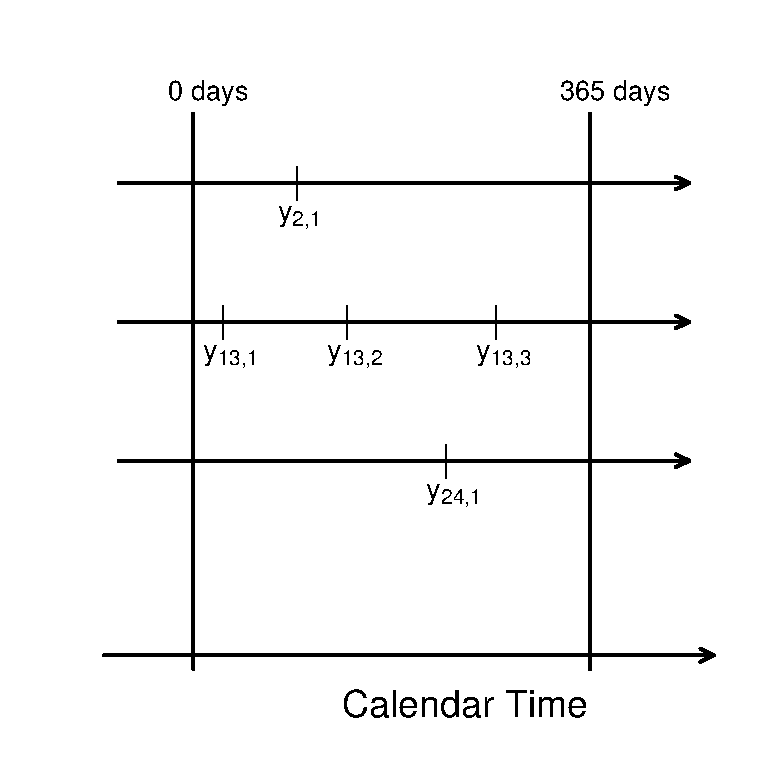
\includegraphics[width=.6\textwidth]{Chapter14Survival/F14Warranty.eps}
    \caption{\label{F14:Warranty}\small Figure Illustrating (Potentially) Repeated Warranty Claims.}
  \end{center}
\end{figure}

\linejed

We present models of recurrent events using \emph{counting
processes}, specifically employ \emph{Poisson processes}. Although
there are alternative approaches, for statistical analyses the
counting process concept seems the most fruitful (Cook and Lawless,
2007). Moreover, there is a strong historical connection of Poisson
processes with actuarial ruin theory (Klugman, Panjer and Willmot,
2008, Chapter 11) and so many actuaries are familiar with Poisson
processes.

Let $N_i(t)$ be the number of events that have occurred by time $t$.
Using algebra, we can write this as $N_i(t) = \sum_{j \geq 1}
\mathrm{I}(y_{ij} \leq t).$ Because $N_i(t)$ varies with a subject's
experience, it is a random variable for each fixed $t$. Further,
when viewing the entire evolution of claims, $\{N_i(t), t \geq 0
\}$, is known as a \emph{stochastic process}. A counting process is
a special kind of stochastic process that describes counts that are
monotonically increasing over time. A Poisson process is a special
kind of counting process. If $\{N_i(t), t \geq 0 \}$ is a Poisson
process, then $N_i(t)$ has a Poisson distribution with mean, say,
$\mathrm{h}_i(t)$ for each fixed $t$. In the counting process
literature, it is customary to refer to $\mathrm{h}_i(t)$ as the
\emph{intensity function}.\index{stochastic process}

Statistical inference for recurrent events can be conducted using
Poisson processes and parametric maximum likelihood techniques. As
discussed in Cook and Lawless (2007), the likelihood for the $i$th
subject is based on the conditional probability density of the
observed outcomes ``$m_i$ events, at times $y_{i1} < \cdots <
y_{im_i}$''. This yields the likelihood
\begin{equation}\label{E14:RecurrLikelihood}
Likelihood_i = \prod_{j=1}^{m_i} \{\mathrm{h}_i(y_{ij}) \} \exp
\left(- \int_0^{\infty} y_i(s) \mathrm{h}_i(s) ds \right)
\end{equation}
where $y_i(s)$ is a binary variable to indicate whether the $i$th
subject is observed by time $s$.

To parameterize the intensity function $\mathrm{h}_i(t)$, we assume
that we have available explanatory variables. For example, when
examining warranty automobile claims, we might have available the
make and model of the vehicle, or driver characteristics such as
gender and age at time of purchase. We might have characteristics
that are functions of the time of claim, such as the number of miles
driven. Thus, we use the notation $\mathbf{x}_i(t)$ to denote the
potential dependence of the explanatory variables on the event time.

Similar to equation (\ref{E14:PHHazardFunction}), it is customary to
write the intensity function as
\begin{equation*}
h_i(t) = h_0(t) \exp( \mathbf{x}_i^{\prime}(t) \boldsymbol \beta ).
\end{equation*}
where $h_0(t)$ is the baseline intensity. For a full parametric
specification, one would specify the baseline intensity in terms of
several parameters. Then, one would use the intensity function
$h_i(t)$ in the likelihood equation (\ref{E14:RecurrLikelihood})
that would serve as the basis for likelihood inference. As discussed
in Cook and Lawless (2007), semi-parametric approaches where the
baseline is not fully parametrically specified (such as the $PH$
model) are also possible.


\section{Further Reading and References}\label{S14:Refer}

As described in Collett (1994), the product-limit estimator had been
used since the early part of the twentieth century. Greenwood (1926)
established the formula for an approximate variance. The work of
Kaplan and Meier (1958) is often associated with the product-limit
estimator; they showed that it is a nonparametric maximum likelihood
estimator of the survival function.

There are several good sources for further study of survival
analysis, particularly in the biomedical sciences; Collett (1994) is
a one such source. The text by Klein and Moeschberger (1997) was
used for several years as required reading for the North American
Society of Actuaries syllabus. Lawless (2003) provides an
introduction from an engineering perspective. Lancaster (1990)
discusses econometric issues. Hougaard (2000) provides an advanced
treatment.

We refer to Cook and Lawless (2007) for a book-long treatment of
recurrent events.

\bigskip

\newpage

\textbf{Chapter References}

\begin{multicols}{2}

\scalefont{0.9}

Breslow, Norman (1974). Covariance analysis of censored survival
data. \textit{Biometrics} 30, 89-99.

Collett, D. (1994). \emph{Modelling Survival Data in Medical
Research.} Chapman \& Hall, London.

Cook, Richard J. and Jerald F. Lawless (2007). \textit{The
Statistical Analysis of Recurrent Events.} Springer-Verlag, New
York.

Cox, David R. (1972). Regression models and life-tables.
\emph{Journal of the Royal Statistical Society, Series B} 34,
187-202.

Gourieroux, Christian and Joann Jasiak (2007). \textit{The
Econometrics of Individual Risk}. Princeton University Press,
Princeton, New Jersey.

Greenwood, M. (1926). The errors of sampling of the survivorship
tables. \textit{Reports on Public Health and Statistical Subjects},
number 33, Appendix, HMSO, London.

Kaplan, E. L. and Meier, P. (1958). Nonparametric estimation from
incomplete observations. \emph{Journal of the American Statistical
Association} 53, 457-481.

Kim, Yong-Duck, Dan R. Anderson, Terry L. Amburgey and James C.
Hickman (1995). The use of event history analysis to examine
insurance insolvencies. \textit{Journal of Risk and Insurance} 62,
94-110.

Klein, John P. and Melvin L. Moeschberger (1997). \textit{Survival
Analysis: Techniques for Censored and Truncated Data}.
Springer-Verlag, New York.

Klugman, Stuart A, Harry H. Panjer and Gordon E. Willmot (2008).
\emph{Loss Models: From Data to Decisions}. John Wiley \& Sons,
Hoboken, New Jersey.

Lancaster, Tony (1990). \textit{The Econometric Analysis of
Transition Data.} Cambridge University Press, New York.

Lawless, Jerald F. (2003). \textit{Statistical Models and Methods
for Lifetime Data, Second Edition.} John Wiley \& Sons, New York.

Hougaard, Philip (2000). \textit{Analysis of Multivariate Survival
Data}. Springer-Verlag, New York.

Miller, Rupert G. (1997). \emph{Survival Analysis}. John Wiley \&
Sons, New York.

Shumway, Tyler (2001). Forecasting bankruptcy more accurately: A
simple hazard model. \textit{Journal of Business} 74, 101-124.

Stepanova, Maria and Lyn Thomas (2002). Survival analysis methods
for personal loan data. \emph{Operations Research} 50(2), 277-290.

Zhou, Mai (2001). Understanding the Cox regression models with
time-changing covariates. \emph{American Statistician} 55(2),
153-155.

\scalefont{1.1111}

\end{multicols}

\bigskip
